\subsection{github}
Lien vers le repository contenant tous les fichiers du projet: \url{https://github.com/mgoretti/HEC-stats}

\subsection{graphiques}
\begin{figure}[H]
\makebox[\textwidth][c]{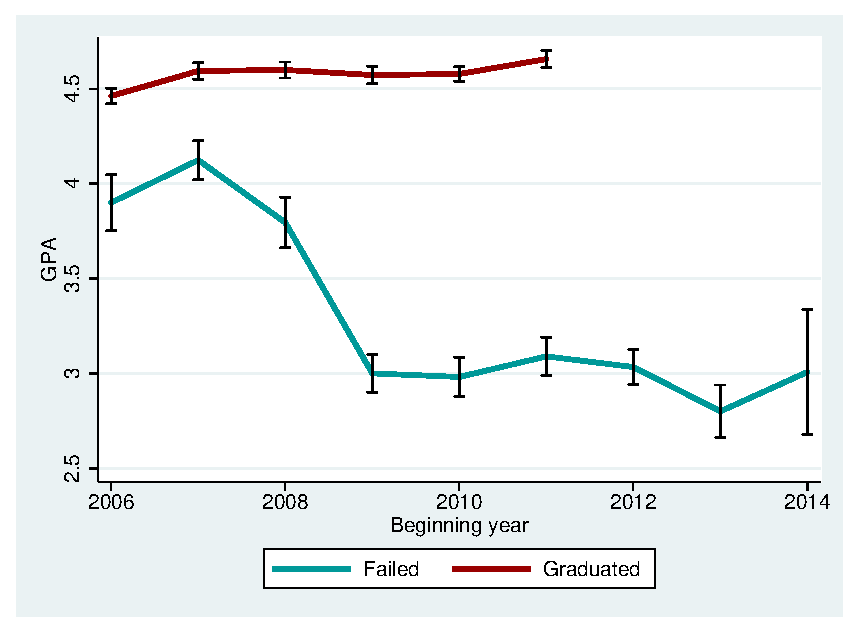
\includegraphics[width=0.6\paperwidth]{img/moyenne.eps}}
\caption{Moyenne par année et par état du cursus (gradué vs. échec/abandon)}
\label{fig:moyenne}
\end{figure}


\begin{figure}[H]
\makebox[\textwidth][c]{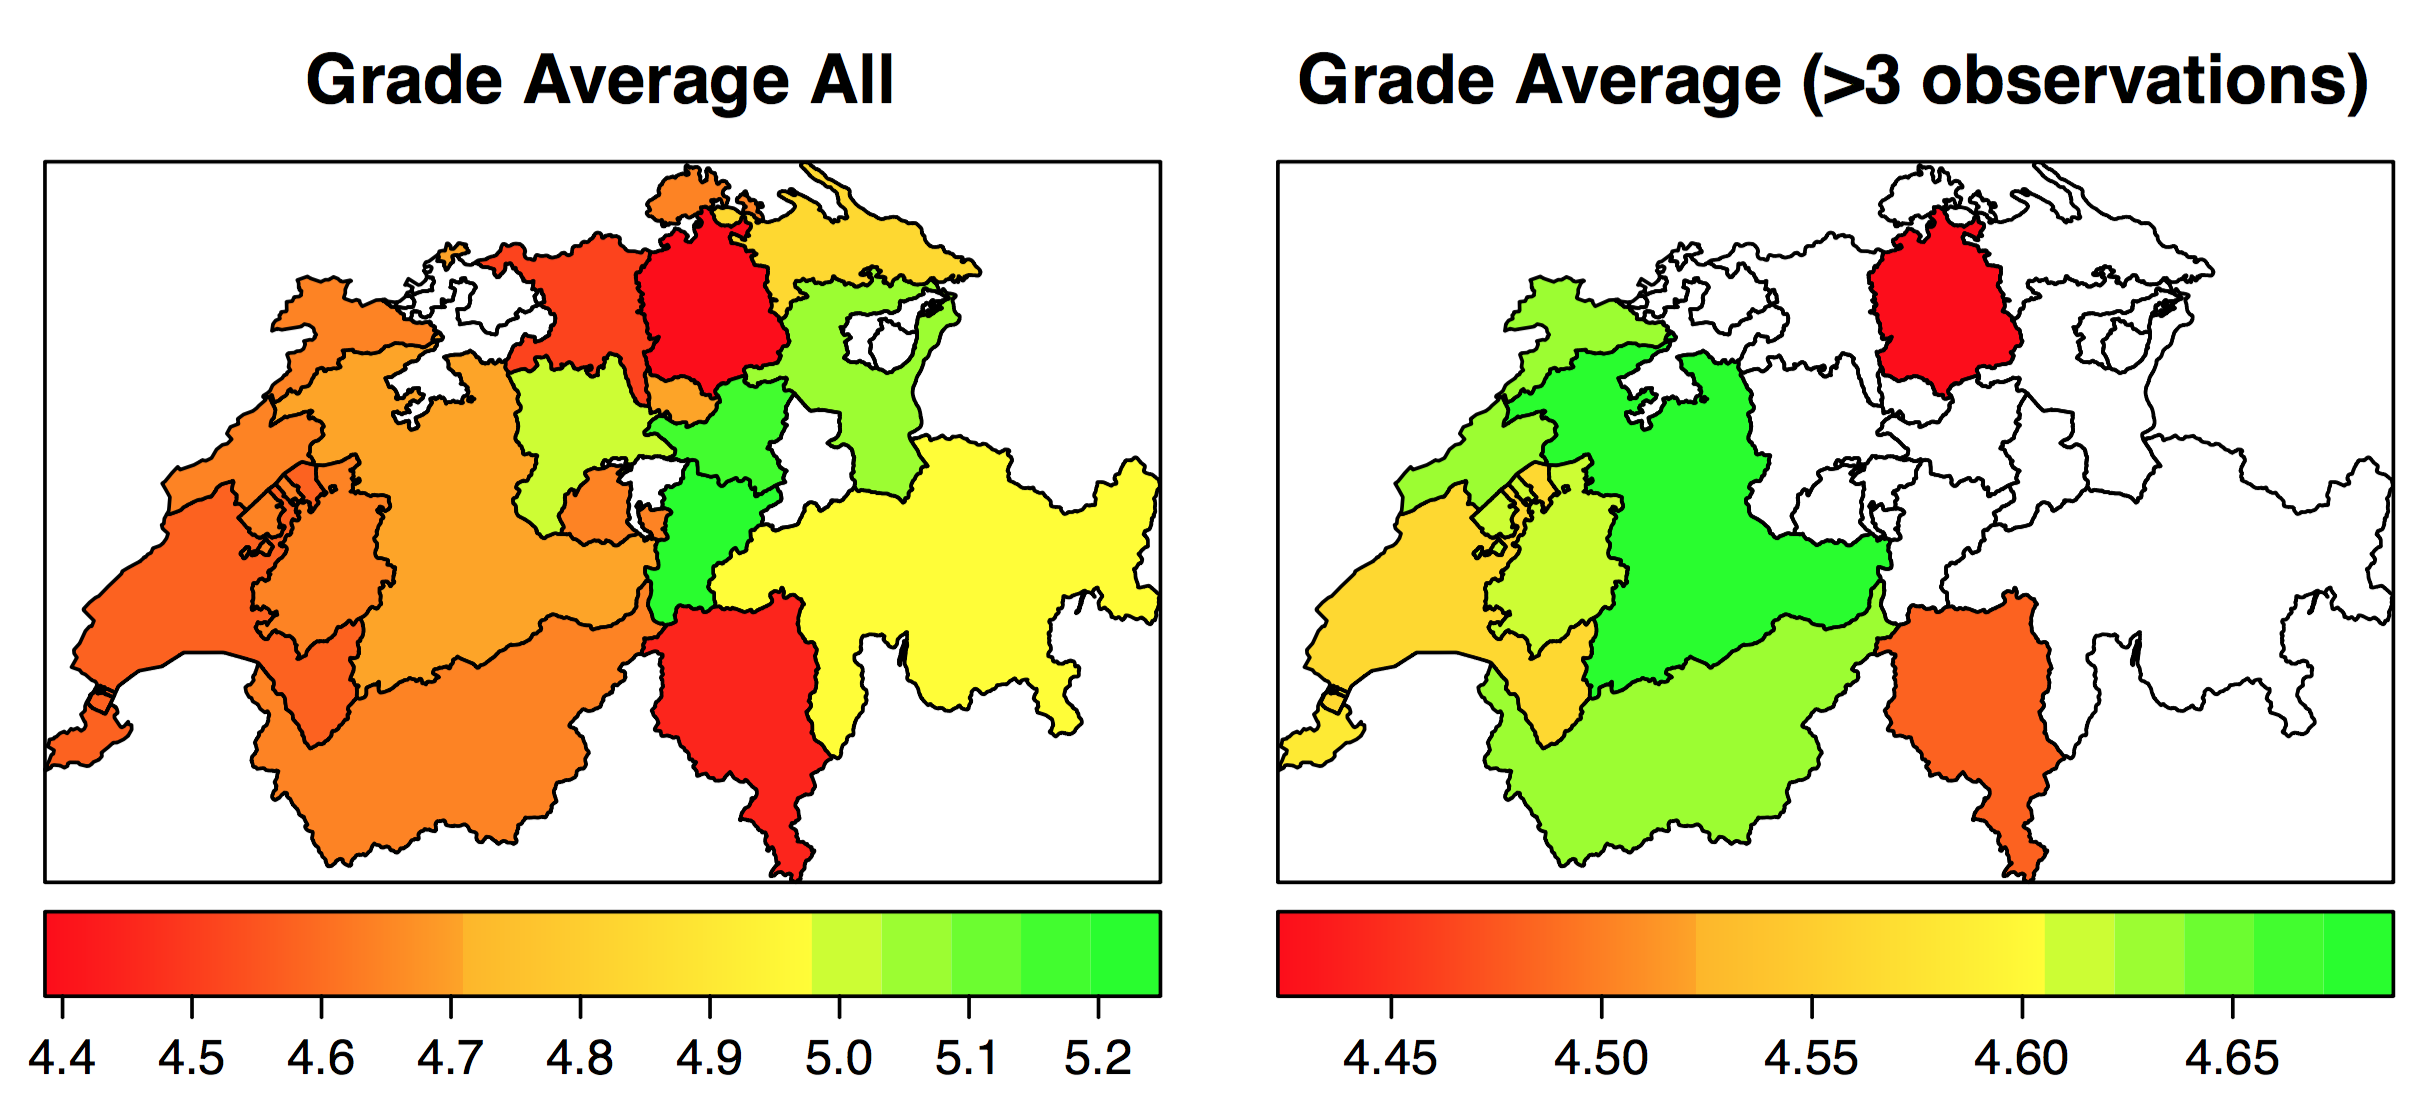
\includegraphics[width=0.9\paperwidth]{img/canton.png}}
\caption{Moyenne au Bachelor par canton de maturité (uniquement cursus réussis)}
\label{fig:canton}
\end{figure}

\begin{figure}[H]
\makebox[\textwidth][c]{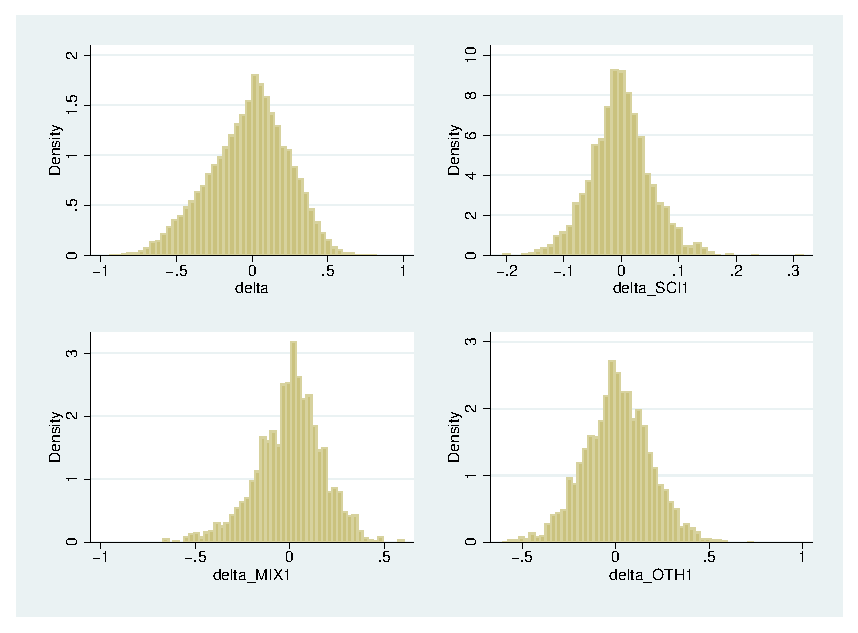
\includegraphics[width=0.75\paperwidth]{img/deltas.eps}}
\caption{Distribution des deltas}
\label{fig:deltas}
\end{figure}

\begin{figure}[H]
\makebox[\textwidth][c]{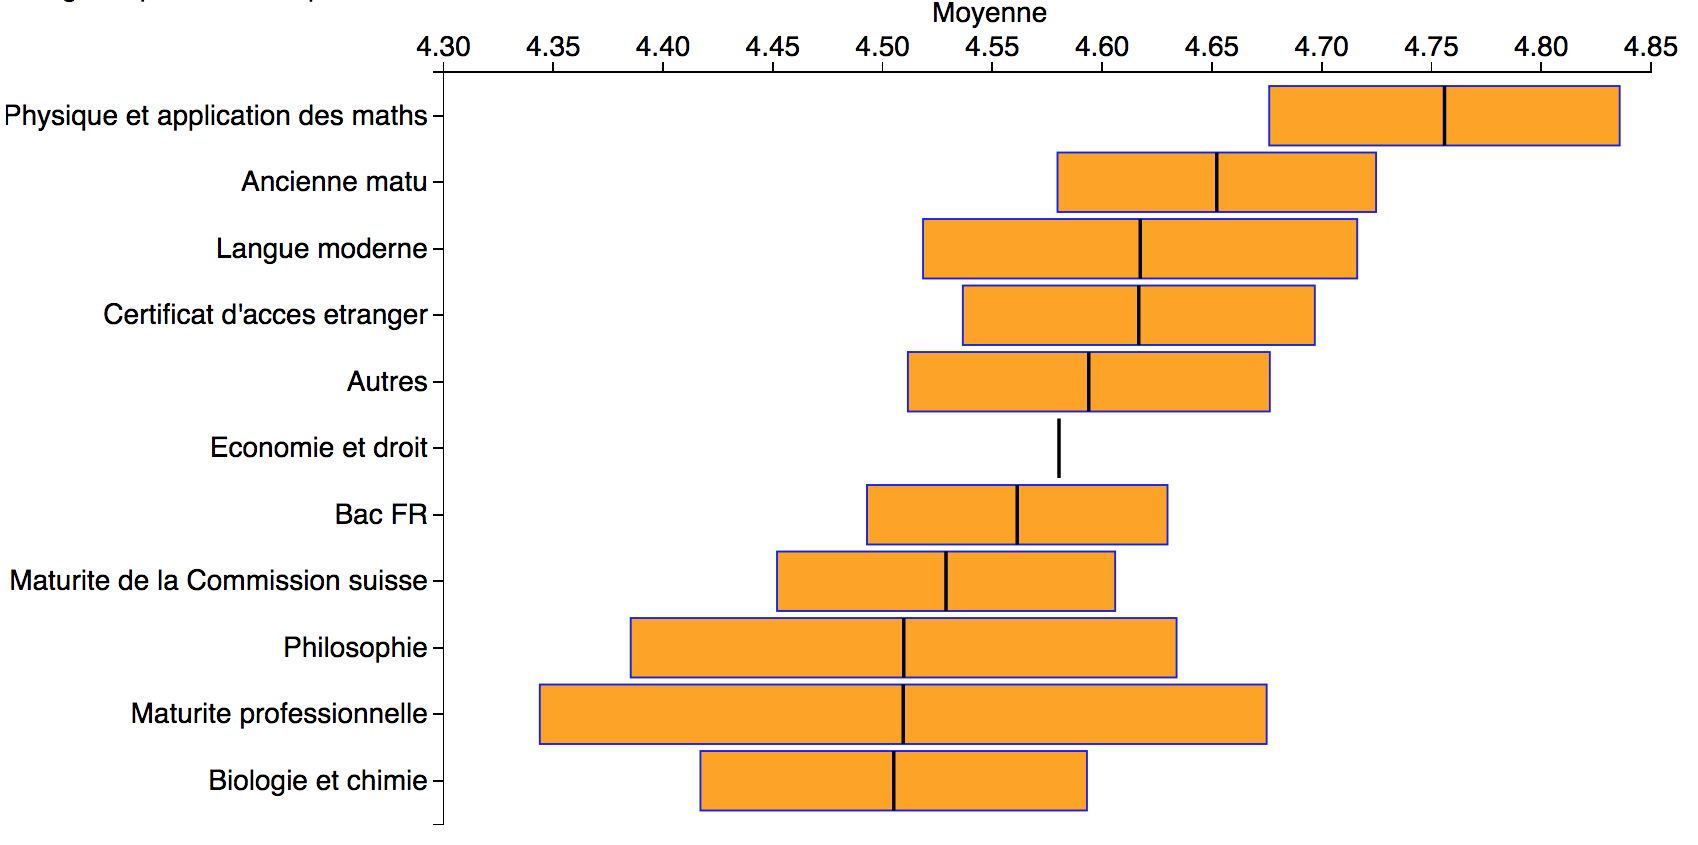
\includegraphics[width=0.8\paperwidth]{img/matu.png}}
\caption{Moyenne au Bachelor par type de maturité (cursus réussis uniquement)}
\label{fig:matu}
\end{figure}

\begin{figure}[H]
\makebox[\textwidth][c]{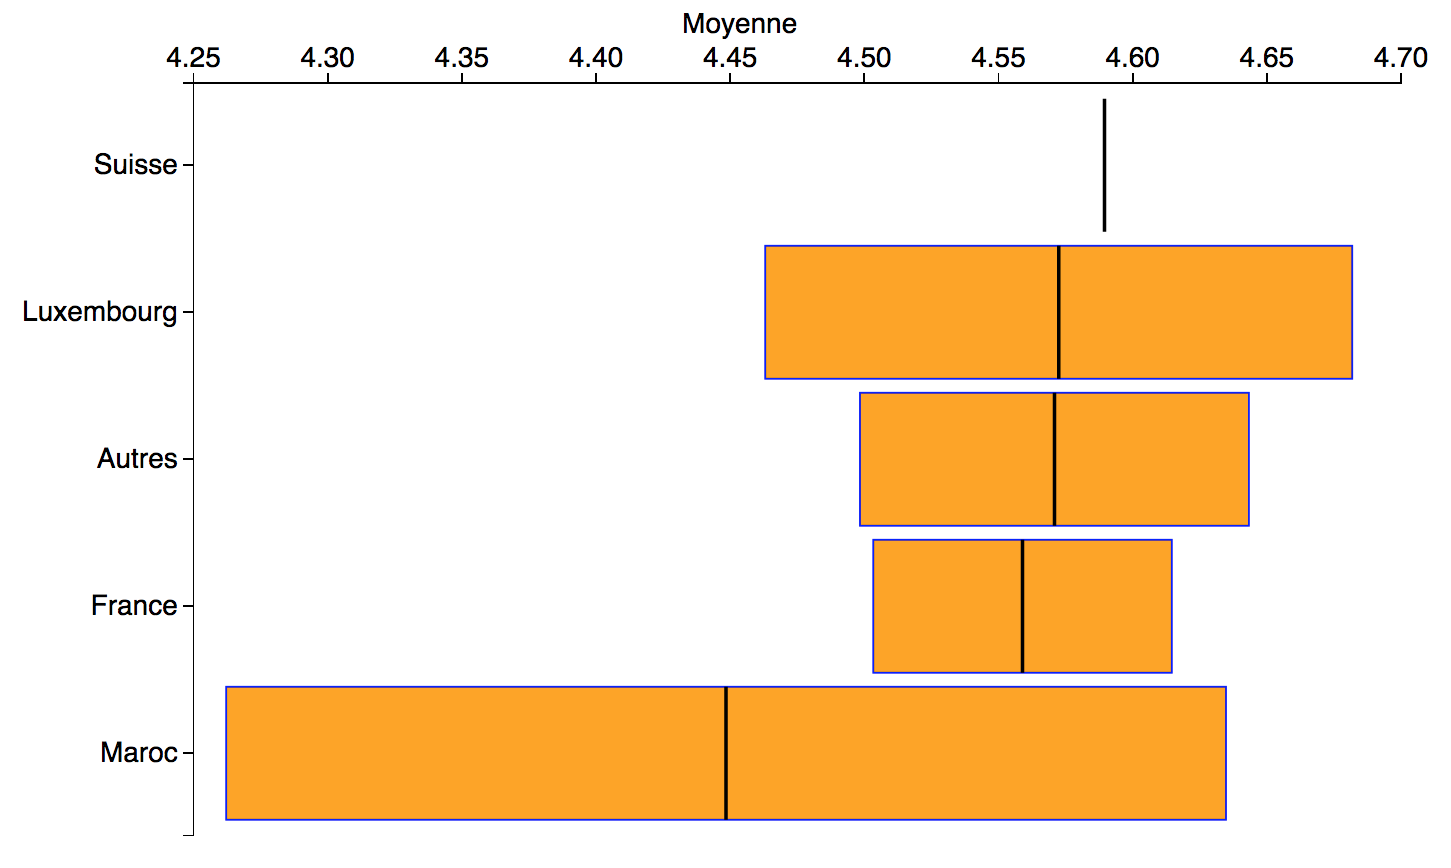
\includegraphics[width=0.95\paperwidth]{img/pays.png}}
\caption{Moyenne au Bachelor par pays d'obtention du diplôme d'accès (cursus réussis uniquement)}
\label{fig:pays}
\end{figure}


\subsection{tableaux}
\subsubsection{Données}

\begin{table}[H]
\begin{center}
\begin{tabular}{l  c  c  c  c  c  c }\hline\hline
\multicolumn{1}{c}{Variables} &delta\_OTH1&delta\_OTH23&delta\_SCI1&delta\_SCI23&delta\_MIX1&delta\_MIX23\\ \hline
delta\_OTH1&1.000\\
delta\_OTH23&0.300&1.000\\
delta\_SCI1&-0.669&-0.184&1.000\\
delta\_SCI23&-0.273&-0.812&0.218&1.000\\
delta\_MIX1&-0.069&-0.042&-0.685&-0.030&1.000\\
delta\_MIX23&-0.095&-0.313&-0.072&-0.080&0.184&1.000\\
\hline \hline 
 \end{tabular}
 \end{center}

\caption{Corrélation entre les delta des différentes catégories}
\label{tab:corr}
\end{table}

\begin{table}[H]
\begin{center}
\begin{tabular}{lcccccc} \hline
 & (1) & (2) & (3) & (4) & (5) & (6) \\
VARIABLES & delta\_SCI23 & delta\_SCI23 & delta\_SCI23 & delta\_SCI23 & delta\_SCI23 & delta\_SCI23 \\ \hline
\vspace{4pt} & \begin{footnotesize}\end{footnotesize} & \begin{footnotesize}\end{footnotesize} & \begin{footnotesize}\end{footnotesize} & \begin{footnotesize}\end{footnotesize} & \begin{footnotesize}\end{footnotesize} & \begin{footnotesize}\end{footnotesize} \\
delta\_SCI1 & 0.339*** &  & 0.066** & 0.207*** &  &  \\
\vspace{4pt} & \begin{footnotesize}(0.032)\end{footnotesize} & \begin{footnotesize}\end{footnotesize} & \begin{footnotesize}(0.032)\end{footnotesize} & \begin{footnotesize}(0.024)\end{footnotesize} & \begin{footnotesize}\end{footnotesize} & \begin{footnotesize}\end{footnotesize} \\
delta\_MIX1 & 0.060*** & -0.016** &  &  & -0.011 &  \\
\vspace{4pt} & \begin{footnotesize}(0.010)\end{footnotesize} & \begin{footnotesize}(0.007)\end{footnotesize} & \begin{footnotesize}\end{footnotesize} & \begin{footnotesize}\end{footnotesize} & \begin{footnotesize}(0.008)\end{footnotesize} & \begin{footnotesize}\end{footnotesize} \\
delta\_OTH1 &  & -0.077*** & -0.062*** &  &  & -0.076*** \\
\vspace{4pt} & \begin{footnotesize}\end{footnotesize} & \begin{footnotesize}(0.007)\end{footnotesize} & \begin{footnotesize}(0.010)\end{footnotesize} & \begin{footnotesize}\end{footnotesize} & \begin{footnotesize}\end{footnotesize} & \begin{footnotesize}(0.007)\end{footnotesize} \\
Constant & -0.015*** & -0.015*** & -0.015*** & -0.016*** & -0.016*** & -0.015*** \\
 & \begin{footnotesize}(0.003)\end{footnotesize} & \begin{footnotesize}(0.003)\end{footnotesize} & \begin{footnotesize}(0.003)\end{footnotesize} & \begin{footnotesize}(0.003)\end{footnotesize} & \begin{footnotesize}(0.003)\end{footnotesize} & \begin{footnotesize}(0.003)\end{footnotesize} \\
\vspace{4pt} & \begin{footnotesize}\end{footnotesize} & \begin{footnotesize}\end{footnotesize} & \begin{footnotesize}\end{footnotesize} & \begin{footnotesize}\end{footnotesize} & \begin{footnotesize}\end{footnotesize} & \begin{footnotesize}\end{footnotesize} \\
Observations & 1,896 & 1,896 & 1,896 & 1,897 & 1,896 & 1,896 \\
 $R^2$ & 0.079 & 0.082 & 0.081 & 0.060 & 0.020 & 0.079 \\ \hline
\multicolumn{7}{c}{\begin{footnotesize} Robust standard errors in parentheses\end{footnotesize}} \\
\multicolumn{7}{c}{\begin{footnotesize} *** p$<$0.01, ** p$<$0.05, * p$<$0.1\end{footnotesize}} \\
\end{tabular}
\end{center}

\caption{Différentes combinaisons de régresseurs expliquant les résultats quantitatifs de 2ème et 3ème année}
\label{tab:sci23}
\end{table}

\begin{table}[H]
\begin{center}
\begin{tabular}{lcccccc} \hline
 & (1) & (2) & (3) & (4) & (5) & (6) \\
VARIABLES & delta\_MIX23 & delta\_MIX23 & delta\_MIX23 & delta\_MIX23 & delta\_MIX23 & delta\_MIX23 \\ \hline
\vspace{4pt} & \begin{footnotesize}\end{footnotesize} & \begin{footnotesize}\end{footnotesize} & \begin{footnotesize}\end{footnotesize} & \begin{footnotesize}\end{footnotesize} & \begin{footnotesize}\end{footnotesize} & \begin{footnotesize}\end{footnotesize} \\
delta\_SCI1 & 0.318*** &  & -0.761*** & -0.245*** &  &  \\
\vspace{4pt} & \begin{footnotesize}(0.112)\end{footnotesize} & \begin{footnotesize}\end{footnotesize} & \begin{footnotesize}(0.112)\end{footnotesize} & \begin{footnotesize}(0.085)\end{footnotesize} & \begin{footnotesize}\end{footnotesize} & \begin{footnotesize}\end{footnotesize} \\
delta\_MIX1 & 0.237*** & 0.168*** &  &  & 0.172*** &  \\
\vspace{4pt} & \begin{footnotesize}(0.033)\end{footnotesize} & \begin{footnotesize}(0.025)\end{footnotesize} & \begin{footnotesize}\end{footnotesize} & \begin{footnotesize}\end{footnotesize} & \begin{footnotesize}(0.025)\end{footnotesize} & \begin{footnotesize}\end{footnotesize} \\
delta\_OTH1 &  & -0.072*** & -0.236*** &  &  & -0.083*** \\
\vspace{4pt} & \begin{footnotesize}\end{footnotesize} & \begin{footnotesize}(0.024)\end{footnotesize} & \begin{footnotesize}(0.033)\end{footnotesize} & \begin{footnotesize}\end{footnotesize} & \begin{footnotesize}\end{footnotesize} & \begin{footnotesize}(0.025)\end{footnotesize} \\
Constant & -0.045*** & -0.044*** & -0.044*** & -0.043*** & -0.044*** & -0.042*** \\
 & \begin{footnotesize}(0.010)\end{footnotesize} & \begin{footnotesize}(0.010)\end{footnotesize} & \begin{footnotesize}(0.010)\end{footnotesize} & \begin{footnotesize}(0.010)\end{footnotesize} & \begin{footnotesize}(0.010)\end{footnotesize} & \begin{footnotesize}(0.010)\end{footnotesize} \\
\vspace{4pt} & \begin{footnotesize}\end{footnotesize} & \begin{footnotesize}\end{footnotesize} & \begin{footnotesize}\end{footnotesize} & \begin{footnotesize}\end{footnotesize} & \begin{footnotesize}\end{footnotesize} & \begin{footnotesize}\end{footnotesize} \\
Observations & 1,485 & 1,485 & 1,485 & 1,486 & 1,485 & 1,485 \\
 $R^2$ & 0.054 & 0.055 & 0.055 & 0.018 & 0.049 & 0.020 \\ \hline
\multicolumn{7}{c}{\begin{footnotesize} Robust standard errors in parentheses\end{footnotesize}} \\
\multicolumn{7}{c}{\begin{footnotesize} *** p$<$0.01, ** p$<$0.05, * p$<$0.1\end{footnotesize}} \\
\end{tabular}
\end{center}

\caption{Différentes combinaisons de régresseurs expliquant les résultats mixtes de 2ème et 3ème année}
\label{tab:mix23}
\end{table}

\begin{table}[H]
\begin{center}
\begin{tabular}{lcccccc} \hline
 & (1) & (2) & (3) & (4) & (5) & (6) \\
VARIABLES & delta\_OTH23 & delta\_OTH23 & delta\_OTH23 & delta\_OTH23 & delta\_OTH23 & delta\_OTH23 \\ \hline
\vspace{4pt} & \begin{footnotesize}\end{footnotesize} & \begin{footnotesize}\end{footnotesize} & \begin{footnotesize}\end{footnotesize} & \begin{footnotesize}\end{footnotesize} & \begin{footnotesize}\end{footnotesize} & \begin{footnotesize}\end{footnotesize} \\
delta\_SCI1 & -0.704*** &  & 0.042 & -0.309*** &  &  \\
\vspace{4pt} & \begin{footnotesize}(0.064)\end{footnotesize} & \begin{footnotesize}\end{footnotesize} & \begin{footnotesize}(0.059)\end{footnotesize} & \begin{footnotesize}(0.045)\end{footnotesize} & \begin{footnotesize}\end{footnotesize} & \begin{footnotesize}\end{footnotesize} \\
delta\_MIX1 & -0.166*** & -0.012 &  &  & -0.021 &  \\
\vspace{4pt} & \begin{footnotesize}(0.019)\end{footnotesize} & \begin{footnotesize}(0.013)\end{footnotesize} & \begin{footnotesize}\end{footnotesize} & \begin{footnotesize}\end{footnotesize} & \begin{footnotesize}(0.013)\end{footnotesize} & \begin{footnotesize}\end{footnotesize} \\
delta\_OTH1 &  & 0.151*** & 0.161*** &  &  & 0.152*** \\
\vspace{4pt} & \begin{footnotesize}\end{footnotesize} & \begin{footnotesize}(0.014)\end{footnotesize} & \begin{footnotesize}(0.019)\end{footnotesize} & \begin{footnotesize}\end{footnotesize} & \begin{footnotesize}\end{footnotesize} & \begin{footnotesize}(0.014)\end{footnotesize} \\
Constant & 0.029*** & 0.028*** & 0.028*** & 0.028*** & 0.028*** & 0.028*** \\
 & \begin{footnotesize}(0.005)\end{footnotesize} & \begin{footnotesize}(0.005)\end{footnotesize} & \begin{footnotesize}(0.005)\end{footnotesize} & \begin{footnotesize}(0.005)\end{footnotesize} & \begin{footnotesize}(0.005)\end{footnotesize} & \begin{footnotesize}(0.005)\end{footnotesize} \\
\vspace{4pt} & \begin{footnotesize}\end{footnotesize} & \begin{footnotesize}\end{footnotesize} & \begin{footnotesize}\end{footnotesize} & \begin{footnotesize}\end{footnotesize} & \begin{footnotesize}\end{footnotesize} & \begin{footnotesize}\end{footnotesize} \\
Observations & 1,504 & 1,504 & 1,504 & 1,505 & 1,504 & 1,504 \\
 $R^2$ & 0.104 & 0.103 & 0.102 & 0.050 & 0.020 & 0.102 \\ \hline
\multicolumn{7}{c}{\begin{footnotesize} Robust standard errors in parentheses\end{footnotesize}} \\
\multicolumn{7}{c}{\begin{footnotesize} *** p$<$0.01, ** p$<$0.05, * p$<$0.1\end{footnotesize}} \\
\end{tabular}
\end{center}

\caption{Différentes combinaisons de régresseurs expliquant les résultats non-quantitatifs de 2ème et 3ème année}
\label{tab:oth23}
\end{table}

\subsubsection{Analyse Descriptive}

\begin{table}[H]
\begin{center}
\begin{tabular}{l|lllllllll|l}
Sex \textbackslash Year & 2006 & 2007 & 2008 & 2009 & 2010 & 2011 & 2012 & 2013 & 2014 & Total \\ \hline
Female                  & 38   & 98   & 100  & 161  & 185  & 160  & 79   & 40   & 7    & 868   \\
Male                    & 69   & 157  & 225  & 307  & 355  & 266  & 141  & 64   & 8    & 1592  \\ \hline
Total                   & 107  & 255  & 325  & 468  & 540  & 426  & 220  & 104  & 15   & 2460 
\end{tabular}
\end{center}
\caption{Nombre d'étudiants par année de début d'études et par sexe}
\label{tab:sex}
\end{table}

\begin{table}[H]
\begin{center}
\begin{tabular}{l|lllllllll|l}
Sex \textbackslash Year & 2006 & 2007 & 2008 & 2009 & 2010 & 2011 & 2012 & 2013 & 2014 & Total \\ \hline
Female                  & 3   & 5   & 25  & 69  & 79  & 75  & 79   & 40   & 7    & 382   \\
Male                    & 0   & 2  & 31  & 111  & 141  & 129  & 141  & 64   & 8    & 627  \\ \hline
Total                   & 3  & 7  & 56  & 180  & 220  & 204  & 220  & 104  & 15   & 1009 
\end{tabular}
\end{center}
\caption{Nombre d'échecs par année de début d'études et par sexe}
\label{tab:echec}
\end{table}

\begin{table}[H]
\begin{center}
\begin{tabular} {@{} l r r r r @{}} \\ \hline
\textbf{debut       stats } & \textbf{  moyenne\_1} & \textbf{  moyenne\_2} & \textbf{  moyenne\_3} & \textbf{   moyenne} \\
\hline
2006         mean  &   4.501402 &   4.279907 &   4.645573 &   4.445414 \\
               sd  &   .2809568 &   .2589845 &    .375799 &   .2272078 \\
2007         mean  &   4.656693 &   4.395773 &   4.731806 &   4.580176 \\
               sd  &   .4055913 &   .3679294 &   .4037419 &   .3494174 \\
2008         mean  &   4.467636 &    4.44772 &   4.729236 &    4.45977 \\
               sd  &   .5248893 &    .401483 &   .3866541 &   .4894625 \\
2009         mean  &   3.942467 &    4.40179 &     4.7692 &   3.967276 \\
               sd  &   .9465355 &   .5682065 &   .4055311 &   .9260684 \\
2010         mean  &   3.890507 &   4.190239 &   4.736133 &   3.927183 \\
               sd  &   .9483145 &   .8016987 &   .4191381 &   .9659944 \\
2011         mean  &   3.900892 &   4.067337 &   4.782489 &   3.905968 \\
               sd  &   .9604512 &    .964434 &    .411499 &   .9663516 \\
2012         mean  &   3.066211 &   2.560022 &          . &    3.03406 \\
               sd  &   .7010399 &   .9965333 &          . &   .6963755 \\
2013         mean  &   2.817063 &   2.565217 &          . &   2.801102 \\
               sd  &   .7278487 &   .9345747 &          . &   .7215713 \\
2014         mean  &   2.974286 &   3.346154 &          . &   3.008039 \\
               sd  &   .6854618 &   .6887372 &          . &   .6485544 \\
Total        mean  &   3.959048 &   4.114521 &   4.740324 &   3.958644 \\
               sd  &   .9401786 &   .8787889 &   .4042057 &   .9303458 \\
\hline
\end{tabular}
\end{center}
\caption{Moyennes générales de l'ensemble des étudiants, par année de début d'études}
\label{tab:moyenne}
\end{table}


\begin{table}[H]
\centering
\resizebox{0.85\textwidth}{!}{\begin{minipage}{\textwidth}%
\begin{center}
\begin{tabular} {@{} l r r r r @{}} \\ \hline
\textbf{debut       stats } & \textbf{  moyenne\_1} & \textbf{  moyenne\_2} & \textbf{  moyenne\_3} & \textbf{   moyenne} \\
\hline
2006         mean  &   4.191667 &   3.683333 &          . &        3.9 \\
               sd  &   .1127314 &   .1626601 &          . &   .1305038 \\
2007         mean  &       4.35 &   3.860714 &          . &    4.12381 \\
               sd  &   .2236068 &   .1398341 &          . &   .1384796 \\
2008         mean  &   3.830003 &     3.6325 &          . &   3.794568 \\
               sd  &   .5310385 &   .5133023 &          . &   .5081951 \\
2009         mean  &   3.006446 &   3.472987 &   3.227273 &   3.000671 \\
               sd  &   .6910325 &   .8823782 &          . &   .6798109 \\
2010         mean  &   2.995184 &   3.172762 &          . &   2.981994 \\
               sd  &   .7931328 &   .9667299 &          . &   .7818877 \\
2011         mean  &   3.118651 &   2.999986 &          . &   3.090132 \\
               sd  &   .7616749 &   .9509751 &          . &   .7387486 \\
2012         mean  &   3.066211 &   2.560022 &          . &    3.03406 \\
               sd  &   .7010399 &   .9965333 &          . &   .6963755 \\
2013         mean  &   2.817063 &   2.565217 &          . &   2.801102 \\
               sd  &   .7278487 &   .9345747 &          . &   .7215713 \\
2014         mean  &   2.974286 &   3.346154 &          . &   3.008039 \\
               sd  &   .6854618 &   .6887372 &          . &   .6485544 \\
Total        mean  &   3.078262 &   2.945794 &   3.227273 &   3.056033 \\
               sd  &   .7601009 &    .996804 &          . &   .7433736 \\
\hline
\end{tabular}
\end{center}

\caption{Moyennes générales des étudiants ayant échoué ou abandonné, \\ par année de début d'études}
\label{tab:moyenneFail}
\end{minipage}}%
\end{table}



\begin{table}[H]
\centering
\resizebox{0.85\textwidth}{!}{\begin{minipage}{\textwidth}%
\begin{center}
\begin{tabular} {@{} l r r r r @{}} \\ \hline
\textbf{debut       stats } & \textbf{  moyenne\_1} & \textbf{  moyenne\_2} & \textbf{  moyenne\_3} & \textbf{   moyenne} \\
\hline
2006         mean  &   4.510337 &   4.297115 &   4.645573 &   4.461147 \\
               sd  &   .2794892 &   .2405156 &    .375799 &   .2094803 \\
2007         mean  &   4.665385 &   4.410876 &   4.731806 &   4.593057 \\
               sd  &   .4064646 &   .3610971 &   .4037419 &   .3449896 \\
2008         mean  &   4.601372 &   4.478026 &   4.729236 &   4.598251 \\
               sd  &    .414312 &   .3641911 &   .3866541 &   .3534436 \\
2009         mean  &   4.527479 &   4.527566 &   4.776948 &   4.571404 \\
               sd  &   .5168007 &   .3613039 &   .3914307 &   .3937089 \\
2010         mean  &   4.506042 &   4.511381 &   4.736133 &   4.577001 \\
               sd  &   .3933755 &   .3493058 &   .4191381 &   .3424582 \\
2011         mean  &   4.619707 &   4.581781 &   4.782489 &   4.655655 \\
               sd  &   .3964997 &   .3595548 &    .411499 &   .3399634 \\
Total        mean  &     4.5728 &   4.486645 &   4.741692 &   4.586304 \\
               sd  &    .424179 &   .3586725 &   .4018165 &   .3500494 \\
\hline
\end{tabular}

\end{center}
\caption{Moyennes générales des étudiants ayant réussi leur cursus, \\ par année de début d'études}
\label{tab:moyenneFini}
\end{minipage}}%
\end{table}

\begin{table}[H]
\begin{center}
\begin{tabular} {@{} l r r r r @{}} \\ \hline
\textbf{   debut } & \textbf{     delta} & \textbf{  delta\_SCI1} & \textbf{  delta\_MIX1} & \textbf{  delta\_OTH1} \\
\hline
2006         mean  &  -.0010201 &   .0024821 &  -.0066845 &  -.0056984 \\
               sd  &   .2549929 &   .0595867 &   .2248986 &   .2106151 \\
2007         mean  &  -.0002217 &   .0033251 &  -.0123725 &  -.0027931 \\
               sd  &   .2473213 &   .0613527 &   .2276017 &   .2038183 \\
2008         mean  &   .0030124 &  -.0043152 &  -.0088202 &   .0274503 \\
               sd  &   .2359713 &   .0615961 &    .212184 &   .1919601 \\
2009         mean  &   .0087136 &  -.0024599 &  -.0028229 &   .0203145 \\
               sd  &   .2219427 &   .0399081 &     .13132 &   .1530087 \\
2010         mean  &   .0014787 &  -.0021758 &   .0145661 &   .0007911 \\
               sd  &   .2264081 &   .0466623 &    .139706 &   .1600304 \\
2011         mean  &  -.0002945 &  -.0014327 &   .0112612 &   -.004182 \\
               sd  &   .2175955 &   .0471209 &   .1463528 &   .1492725 \\
2012         mean  &   .0035528 &  -.0053011 &  -.0029394 &   .0291159 \\
               sd  &   .2043771 &   .0543845 &   .1486076 &   .1844625 \\
2013         mean  &   .0053406 &  -.0074005 &  -.0127259 &   .0471383 \\
               sd  &   .2135919 &   .0563327 &   .1876084 &    .191214 \\
2014         mean  &  -.0032677 &   .0040687 &  -.0318605 &  -.0064318 \\
               sd  &   .1876941 &   .0792771 &   .2254533 &   .2605538 \\
Total        mean  &    .002515 &  -.0016027 &   .0011797 &    .008531 \\
               sd  &   .2292595 &   .0516892 &   .1730637 &   .1740549 \\
\hline

\end{tabular}
\end{center}
\caption{Distribution des différents delta par année de début d'études}
\label{tab:deltas}
\end{table}

\subsubsection{Résultats}

\begin{table}[H]
  \centering
  %\setcapwidth{0.6\textwidth}
  \checkoddpage
  \edef\side{\ifoddpage l\else r\fi}%
\resizebox{0.85\textwidth}{!}{
    \begin{minipage}[t]{.45\textwidth}
      \centering
      \begin{center}
\begin{tabular}{lcc} \hline
 & (1) & (2) \\
& quant\_2 & moyenne\_2 \\ \hline
\vspace{4pt} & \begin{footnotesize}\end{footnotesize} & \begin{footnotesize}\end{footnotesize} \\
delta\_SCI1 & 0.485*** & 1.272*** \\
\vspace{4pt} & \begin{footnotesize}(0.116)\end{footnotesize} & \begin{footnotesize}(0.384)\end{footnotesize} \\
delta\_MIX1 & 0.180*** & 0.501*** \\
\vspace{4pt} & \begin{footnotesize}(0.032)\end{footnotesize} & \begin{footnotesize}(0.105)\end{footnotesize} \\
Sexe = 2, M & -0.006 & -0.004 \\
\vspace{4pt} & \begin{footnotesize}(0.010)\end{footnotesize} & \begin{footnotesize}(0.035)\end{footnotesize} \\
Constant & 0.548*** & 4.191*** \\
 & \begin{footnotesize}(0.013)\end{footnotesize} & \begin{footnotesize}(0.048)\end{footnotesize} \\
\vspace{4pt} & \begin{footnotesize}\end{footnotesize} & \begin{footnotesize}\end{footnotesize} \\
Control: Year & Yes & Yes \\ \hline
Observations & 1,909 & 1,909 \\
 $R^2$ & 0.031 & 0.365 \\ \hline
\multicolumn{3}{c}{\begin{footnotesize} Robust standard errors in parentheses\end{footnotesize}} \\
\multicolumn{3}{c}{\begin{footnotesize} *** p$<$0.01, ** p$<$0.05, * p$<$0.1\end{footnotesize}} \\
\end{tabular}
\end{center}

	  \caption{Effets de la surperformance 
      catégorielle \\ sur la moyenne relative et 
      absolue de deuxième \\ année}
      \label{tab:result2}

    \end{minipage}%
    \hfill
    \begin{minipage}[t]{0.45\textwidth}
      \centering
      \begin{center}
\begin{tabular}{lcc} \hline
 & (1) & (2) \\
& quant\_3 & moyenne\_3 \\ \hline
\vspace{4pt} & \begin{footnotesize}\end{footnotesize} & \begin{footnotesize}\end{footnotesize} \\
delta\_SCI1 & -0.258** & -0.264 \\
\vspace{4pt} & \begin{footnotesize}(0.123)\end{footnotesize} & \begin{footnotesize}(0.317)\end{footnotesize} \\
delta\_MIX1 & -0.051 & -0.059 \\
\vspace{4pt} & \begin{footnotesize}(0.035)\end{footnotesize} & \begin{footnotesize}(0.087)\end{footnotesize} \\
Sexe = 2, M & -0.036*** & -0.071*** \\
\vspace{4pt} & \begin{footnotesize}(0.010)\end{footnotesize} & \begin{footnotesize}(0.025)\end{footnotesize} \\
Constant & 0.659*** & 4.783*** \\
 & \begin{footnotesize}(0.012)\end{footnotesize} & \begin{footnotesize}(0.031)\end{footnotesize} \\
\vspace{4pt} & \begin{footnotesize}\end{footnotesize} & \begin{footnotesize}\end{footnotesize} \\
Control: Year & Yes & Yes \\ \hline
Observations & 1,103 & 1,103 \\
 $R^2$ & 0.026 & 0.015 \\ \hline
\multicolumn{3}{c}{\begin{footnotesize} Robust standard errors in parentheses\end{footnotesize}} \\
\multicolumn{3}{c}{\begin{footnotesize} *** p$<$0.01, ** p$<$0.05, * p$<$0.1\end{footnotesize}} \\
\end{tabular}
\end{center}

	  \caption{Effets de la surperformance
      catégorielle \\ sur la moyenne relative et 
      absolue de troisième \\ année}
      \label{tab:result3}
    \end{minipage}%
  }%

\end{table}


\begin{table}[H]
\centering
\resizebox{0.85\textwidth}{!}{\begin{minipage}{\textwidth}%
\begin{center}
\begin{tabular}{lcccccc} \hline
 & (1) & (2) & (3) & (4) & (5) & (6) \\
VARIABLES & quant\_2 & quant\_2 & quant\_2 & quant\_2 & quant\_2 & quant\_2 \\ \hline
\vspace{4pt} & \begin{footnotesize}\end{footnotesize} & \begin{footnotesize}\end{footnotesize} & \begin{footnotesize}\end{footnotesize} & \begin{footnotesize}\end{footnotesize} & \begin{footnotesize}\end{footnotesize} & \begin{footnotesize}\end{footnotesize} \\
delta\_SCI1 & 0.485*** &  & -0.312*** & 0.085 &  &  \\
\vspace{4pt} & \begin{footnotesize}(0.116)\end{footnotesize} & \begin{footnotesize}\end{footnotesize} & \begin{footnotesize}(0.106)\end{footnotesize} & \begin{footnotesize}(0.083)\end{footnotesize} & \begin{footnotesize}\end{footnotesize} & \begin{footnotesize}\end{footnotesize} \\
delta\_MIX1 & 0.180*** & 0.073*** &  &  & 0.079*** &  \\
\vspace{4pt} & \begin{footnotesize}(0.032)\end{footnotesize} & \begin{footnotesize}(0.023)\end{footnotesize} & \begin{footnotesize}\end{footnotesize} & \begin{footnotesize}\end{footnotesize} & \begin{footnotesize}(0.023)\end{footnotesize} & \begin{footnotesize}\end{footnotesize} \\
delta\_OTH1 &  & -0.108*** & -0.176*** &  &  & -0.111*** \\
\vspace{4pt} & \begin{footnotesize}\end{footnotesize} & \begin{footnotesize}(0.025)\end{footnotesize} & \begin{footnotesize}(0.032)\end{footnotesize} & \begin{footnotesize}\end{footnotesize} & \begin{footnotesize}\end{footnotesize} & \begin{footnotesize}(0.025)\end{footnotesize} \\
Constant & 0.548*** & 0.548*** & 0.549*** & 0.547*** & 0.546*** & 0.549*** \\
 & \begin{footnotesize}(0.013)\end{footnotesize} & \begin{footnotesize}(0.013)\end{footnotesize} & \begin{footnotesize}(0.013)\end{footnotesize} & \begin{footnotesize}(0.013)\end{footnotesize} & \begin{footnotesize}(0.013)\end{footnotesize} & \begin{footnotesize}(0.013)\end{footnotesize} \\
\vspace{4pt} & \begin{footnotesize}\end{footnotesize} & \begin{footnotesize}\end{footnotesize} & \begin{footnotesize}\end{footnotesize} & \begin{footnotesize}\end{footnotesize} & \begin{footnotesize}\end{footnotesize} & \begin{footnotesize}\end{footnotesize} \\
Observations & 1,909 & 1,909 & 1,909 & 1,910 & 1,909 & 1,909 \\
 $R^2$ & 0.031 & 0.031 & 0.030 & 0.019 & 0.023 & 0.027 \\ \hline
\multicolumn{7}{c}{\begin{footnotesize} Robust standard errors in parentheses\end{footnotesize}} \\
\multicolumn{7}{c}{\begin{footnotesize} *** p$<$0.01, ** p$<$0.05, * p$<$0.1\end{footnotesize}} \\
\end{tabular}
\end{center}

\caption{Toutes les combinaisons de régresseurs pour (1) du tableau \ref{tab:result2}}
\label{tab:quant2}
\end{minipage}}%
\end{table}


\begin{table}[H]
\begin{center}
\begin{tabular}{lccc} \hline
 & (1) & (2) & (3) \\
VARIABLES & fini & fini & y1 \\ \hline
\vspace{4pt} & \begin{footnotesize}\end{footnotesize} & \begin{footnotesize}\end{footnotesize} & \begin{footnotesize}\end{footnotesize} \\
delta\_SCI1 & 10.372*** &  &  \\
\vspace{4pt} & \begin{footnotesize}(1.456)\end{footnotesize} & \begin{footnotesize}\end{footnotesize} & \begin{footnotesize}\end{footnotesize} \\
delta\_MIX1 & 3.522*** &  &  \\
\vspace{4pt} & \begin{footnotesize}(0.461)\end{footnotesize} & \begin{footnotesize}\end{footnotesize} & \begin{footnotesize}\end{footnotesize} \\
Debut = 2006 & 3.604*** & 3.530*** & 0.455*** \\
\vspace{4pt} & \begin{footnotesize}(0.601)\end{footnotesize} & \begin{footnotesize}(0.596)\end{footnotesize} & \begin{footnotesize}(0.030)\end{footnotesize} \\
Debut = 2007 & 3.614*** & 3.536*** & 0.455*** \\
\vspace{4pt} & \begin{footnotesize}(0.403)\end{footnotesize} & \begin{footnotesize}(0.403)\end{footnotesize} & \begin{footnotesize}(0.028)\end{footnotesize} \\
Debut = 2008 & 1.640*** & 1.593*** & 0.322*** \\
\vspace{4pt} & \begin{footnotesize}(0.185)\end{footnotesize} & \begin{footnotesize}(0.182)\end{footnotesize} & \begin{footnotesize}(0.033)\end{footnotesize} \\
Debut = 2009 & 0.471*** & 0.454*** & 0.110*** \\
\vspace{4pt} & \begin{footnotesize}(0.141)\end{footnotesize} & \begin{footnotesize}(0.140)\end{footnotesize} & \begin{footnotesize}(0.034)\end{footnotesize} \\
Debut = 2010 & 0.357*** & 0.361*** & 0.089*** \\
\vspace{4pt} & \begin{footnotesize}(0.137)\end{footnotesize} & \begin{footnotesize}(0.136)\end{footnotesize} & \begin{footnotesize}(0.033)\end{footnotesize} \\
Debut = 2012, omitted & - & - & - \\
\vspace{4pt} & \begin{footnotesize}\end{footnotesize} & \begin{footnotesize}\end{footnotesize} & \begin{footnotesize}\end{footnotesize} \\
Debut = 2013, omitted & - & - & - \\
\vspace{4pt} & \begin{footnotesize}\end{footnotesize} & \begin{footnotesize}\end{footnotesize} & \begin{footnotesize}\end{footnotesize} \\
Debut = 2014, omitted & - & - & - \\
\vspace{4pt} & \begin{footnotesize}\end{footnotesize} & \begin{footnotesize}\end{footnotesize} & \begin{footnotesize}\end{footnotesize} \\
delta\_OTH1 &  & -2.378*** & -0.441*** \\
\vspace{4pt} & \begin{footnotesize}\end{footnotesize} & \begin{footnotesize}(0.300)\end{footnotesize} & \begin{footnotesize}(0.055)\end{footnotesize} \\
Constant & 0.102 & 0.120 &  \\
 & \begin{footnotesize}(0.104)\end{footnotesize} & \begin{footnotesize}(0.103)\end{footnotesize} & \begin{footnotesize}\end{footnotesize} \\
\vspace{4pt} & \begin{footnotesize}\end{footnotesize} & \begin{footnotesize}\end{footnotesize} & \begin{footnotesize}\end{footnotesize} \\
 Observations & 2,103 & 2,102 & 2,102 \\ \hline
\multicolumn{4}{c}{\begin{footnotesize} Robust standard errors in parentheses\end{footnotesize}} \\
\multicolumn{4}{c}{\begin{footnotesize} *** p$<$0.01, ** p$<$0.05, * p$<$0.1\end{footnotesize}} \\
\end{tabular}
\end{center}

\caption{Probabilité de réussir en fonction des deltas. Référence: début en 2011}
\label{tab:logit}
\end{table}

\begin{table}[H]
  %\setcapwidth{0.6\textwidth}
  \checkoddpage
  \edef\side{\ifoddpage l\else r\fi}%
  \makebox[\textwidth][\side]{%
    \begin{minipage}[t]{.5\textwidth}
      \centering
      \begin{center}
\begin{tabular}{lc} \hline
 & (1) \\
 & quant 2 \\ \hline
\vspace{4pt} & \begin{footnotesize}\end{footnotesize} \\
Management & -0.061*** \\
\vspace{4pt} & \begin{footnotesize}(0.022)\end{footnotesize} \\
Maths & 0.104*** \\
\vspace{4pt} & \begin{footnotesize}(0.039)\end{footnotesize} \\
Compta & 0.127*** \\
\vspace{4pt} & \begin{footnotesize}(0.031)\end{footnotesize} \\
Constant & 0.604*** \\
 & \begin{footnotesize}(0.009)\end{footnotesize} \\
\vspace{4pt} & \begin{footnotesize}\end{footnotesize} \\
Observations & 951 \\
 $R^2$ & 0.042 \\ \hline
\multicolumn{2}{c}{\begin{footnotesize} Robust standard errors in parentheses\end{footnotesize}} \\
\multicolumn{2}{c}{\begin{footnotesize} *** p$<$0.01, ** p$<$0.05, * p$<$0.1\end{footnotesize}} \\
\end{tabular}
\end{center}
	  \caption{Effet de la surperformance par cours de première année sur la moyenne normalisée de deuxième (Plans d'études à examens annuels, avant 2011)}
      \label{tab:oldClasses}

    \end{minipage}%
    \hfill
    \begin{minipage}[t]{0.5\textwidth}
      \centering
      \begin{center}
\begin{tabular}{lc} \hline
 & (1) \\
 & quant 2 \\ \hline
\vspace{4pt} & \begin{footnotesize}\end{footnotesize} \\
Management & -0.037 \\
\vspace{4pt} & \begin{footnotesize}(0.047)\end{footnotesize} \\
compta I & -0.176*** \\
\vspace{4pt} & \begin{footnotesize}(0.059)\end{footnotesize} \\
compta II & 0.122** \\
\vspace{4pt} & \begin{footnotesize}(0.057)\end{footnotesize} \\
Prog & -0.143** \\
\vspace{4pt} & \begin{footnotesize}(0.063)\end{footnotesize} \\
Droit 1er & -0.209*** \\
\vspace{4pt} & \begin{footnotesize}(0.046)\end{footnotesize} \\
Droit 2e & 0.033 \\
\vspace{4pt} & \begin{footnotesize}(0.051)\end{footnotesize} \\
Modeles Info & -0.252*** \\
\vspace{4pt} & \begin{footnotesize}(0.062)\end{footnotesize} \\
Stats I & -0.130** \\
\vspace{4pt} & \begin{footnotesize}(0.057)\end{footnotesize} \\
Stats II & 0.089 \\
\vspace{4pt} & \begin{footnotesize}(0.060)\end{footnotesize} \\
Constant & 0.610*** \\
 & \begin{footnotesize}(0.017)\end{footnotesize} \\
\vspace{4pt} & \begin{footnotesize}\end{footnotesize} \\
Observations & 551 \\
 $R^2$ & 0.175 \\ \hline
\multicolumn{2}{c}{\begin{footnotesize} Robust standard errors in parentheses\end{footnotesize}} \\
\multicolumn{2}{c}{\begin{footnotesize} *** p$<$0.01, ** p$<$0.05, * p$<$0.1\end{footnotesize}} \\
\end{tabular}
\end{center}
	  \caption{Effet de la surperformance par cours de première année sur la moyenne normalisée de deuxième (Plans d'études à examens semestriels, dès 2011)}
      \label{tab:newClasses}
    \end{minipage}%
  }%
\end{table}

\begin{table}[H]
\centering
\resizebox{0.85\textwidth}{!}{\begin{minipage}{\textwidth}%
\begin{center}
\begin{tabular}{lcc} \hline
 & (1) & (2) \\
 & moyenne 2e & moyenne 3e \\ \hline
\vspace{4pt} & \begin{footnotesize}\end{footnotesize} & \begin{footnotesize}\end{footnotesize} \\
Male & -0.030 & -0.088*** \\
\vspace{4pt} & \begin{footnotesize}(0.029)\end{footnotesize} & \begin{footnotesize}(0.024)\end{footnotesize} \\
Echec. & -1.484*** &  \\
\vspace{4pt} & \begin{footnotesize}(0.047)\end{footnotesize} & \begin{footnotesize}\end{footnotesize} \\
Bach. Eco. & 0.273*** & 0.223*** \\
\vspace{4pt} & \begin{footnotesize}(0.025)\end{footnotesize} & \begin{footnotesize}(0.034)\end{footnotesize} \\
Constant & 4.443*** & 4.757*** \\
 & \begin{footnotesize}(0.020)\end{footnotesize} & \begin{footnotesize}(0.019)\end{footnotesize} \\
\vspace{4pt} & \begin{footnotesize}\end{footnotesize} & \begin{footnotesize}\end{footnotesize} \\
Observations & 1,913 & 1,107 \\
 $R^2$ & 0.579 & 0.053 \\ \hline
\multicolumn{3}{c}{\begin{footnotesize} Robust standard errors in parentheses\end{footnotesize}} \\
\multicolumn{3}{c}{\begin{footnotesize} *** p$<$0.01, ** p$<$0.05, * p$<$0.1\end{footnotesize}} \\
\end{tabular}
\end{center}
\caption{Distinction entre les orientations de troisième année (référence: Management)}
\label{tab:bac}
\end{minipage}}%
\end{table}

\begin{table}[H]
\centering
\resizebox{0.85\textwidth}{!}{\begin{minipage}{\textwidth}%
\begin{center}
\begin{tabular}{lcccc} \hline
 & (1) & (2) & (3) & (4) \\
Moyenne & Tous & Tous & Bachelor réussi & Bachelor réussi \\ \hline
\vspace{4pt} & \begin{footnotesize}\end{footnotesize} & \begin{footnotesize}\end{footnotesize} & \begin{footnotesize}\end{footnotesize} & \begin{footnotesize}\end{footnotesize} \\
Male & 0.052 & 0.048 & 0.004 & 0.006 \\
\vspace{4pt} & \begin{footnotesize}(0.039)\end{footnotesize} & \begin{footnotesize}(0.034)\end{footnotesize} & \begin{footnotesize}(0.019)\end{footnotesize} & \begin{footnotesize}(0.019)\end{footnotesize} \\
Autres & -0.479*** & -0.311*** & -0.020 & -0.019 \\
\vspace{4pt} & \begin{footnotesize}(0.084)\end{footnotesize} & \begin{footnotesize}(0.072)\end{footnotesize} & \begin{footnotesize}(0.038)\end{footnotesize} & \begin{footnotesize}(0.037)\end{footnotesize} \\
France & -0.250*** & -0.143*** & -0.029 & -0.031 \\
\vspace{4pt} & \begin{footnotesize}(0.054)\end{footnotesize} & \begin{footnotesize}(0.046)\end{footnotesize} & \begin{footnotesize}(0.029)\end{footnotesize} & \begin{footnotesize}(0.028)\end{footnotesize} \\
Luxembourg & -0.136 & -0.118 & -0.004 & -0.017 \\
\vspace{4pt} & \begin{footnotesize}(0.137)\end{footnotesize} & \begin{footnotesize}(0.133)\end{footnotesize} & \begin{footnotesize}(0.055)\end{footnotesize} & \begin{footnotesize}(0.056)\end{footnotesize} \\
Maroc & -0.944*** & -0.627*** & -0.166* & -0.141 \\
\vspace{4pt} & \begin{footnotesize}(0.125)\end{footnotesize} & \begin{footnotesize}(0.116)\end{footnotesize} & \begin{footnotesize}(0.096)\end{footnotesize} & \begin{footnotesize}(0.095)\end{footnotesize} \\
Constant & 4.021*** & 3.963*** & 4.590*** & 4.581*** \\
 & \begin{footnotesize}(0.033)\end{footnotesize} & \begin{footnotesize}(0.047)\end{footnotesize} & \begin{footnotesize}(0.017)\end{footnotesize} & \begin{footnotesize}(0.024)\end{footnotesize} \\
\vspace{4pt} & \begin{footnotesize}\end{footnotesize} & \begin{footnotesize}\end{footnotesize} & \begin{footnotesize}\end{footnotesize} & \begin{footnotesize}\end{footnotesize} \\
Control: Year & No & Yes & No & Yes \\ \hline
Observations & 2,460 & 2,460 & 1,451 & 1,451 \\
 $R^2$ & 0.046 & 0.277 & 0.003 & 0.018 \\ \hline
\multicolumn{5}{c}{\begin{footnotesize} Robust standard errors in parentheses\end{footnotesize}} \\
\multicolumn{5}{c}{\begin{footnotesize} *** p$<$0.01, ** p$<$0.05, * p$<$0.1\end{footnotesize}} \\
\end{tabular}
\end{center}

\caption{Moyenne (avec et sans échecs) en fonction du pays de maturité. Référence: Suisse, 2010}
\label{tab:matuLieu}
\end{minipage}}%
\end{table}

\begin{table}[H]
\begin{center}
\begin{tabular}{lcccc} \hline
 & (1) & (2) & (3) & (4) \\
Moyenne & Tous & Tous & Bachelor réussi & Bachelor réussi \\ \hline
\vspace{4pt} & \begin{footnotesize}\end{footnotesize} & \begin{footnotesize}\end{footnotesize} & \begin{footnotesize}\end{footnotesize} & \begin{footnotesize}\end{footnotesize} \\
Male & 0.015 & 0.017 & -0.003 & -0.002 \\
\vspace{4pt} & \begin{footnotesize}(0.037)\end{footnotesize} & \begin{footnotesize}(0.034)\end{footnotesize} & \begin{footnotesize}(0.019)\end{footnotesize} & \begin{footnotesize}(0.019)\end{footnotesize} \\
Autres & -0.563*** & -0.420*** & 0.002 & 0.014 \\
\vspace{4pt} & \begin{footnotesize}(0.085)\end{footnotesize} & \begin{footnotesize}(0.077)\end{footnotesize} & \begin{footnotesize}(0.043)\end{footnotesize} & \begin{footnotesize}(0.042)\end{footnotesize} \\
Bac FR & -0.593*** & -0.394*** & -0.017 & -0.019 \\
\vspace{4pt} & \begin{footnotesize}(0.060)\end{footnotesize} & \begin{footnotesize}(0.057)\end{footnotesize} & \begin{footnotesize}(0.035)\end{footnotesize} & \begin{footnotesize}(0.035)\end{footnotesize} \\
Certificat d'accès étranger & 0.254*** & -0.319*** & -0.006 & 0.036 \\
\vspace{4pt} & \begin{footnotesize}(0.059)\end{footnotesize} & \begin{footnotesize}(0.064)\end{footnotesize} & \begin{footnotesize}(0.034)\end{footnotesize} & \begin{footnotesize}(0.041)\end{footnotesize} \\
Diplôme de fin d'études secondaires & -0.257 & -0.196 & 0.002 & -0.012 \\
\vspace{4pt} & \begin{footnotesize}(0.164)\end{footnotesize} & \begin{footnotesize}(0.165)\end{footnotesize} & \begin{footnotesize}(0.066)\end{footnotesize} & \begin{footnotesize}(0.066)\end{footnotesize} \\
Maturité de la Commission suisse & -0.393*** & -0.474*** & -0.067* & -0.051 \\
\vspace{4pt} & \begin{footnotesize}(0.079)\end{footnotesize} & \begin{footnotesize}(0.072)\end{footnotesize} & \begin{footnotesize}(0.038)\end{footnotesize} & \begin{footnotesize}(0.039)\end{footnotesize} \\
Biologie et chimie & -0.270*** & -0.195** & -0.076* & -0.075* \\
\vspace{4pt} & \begin{footnotesize}(0.085)\end{footnotesize} & \begin{footnotesize}(0.079)\end{footnotesize} & \begin{footnotesize}(0.045)\end{footnotesize} & \begin{footnotesize}(0.045)\end{footnotesize} \\
Langue moderne & -0.314*** & -0.220*** & 0.037 & 0.037 \\
\vspace{4pt} & \begin{footnotesize}(0.095)\end{footnotesize} & \begin{footnotesize}(0.084)\end{footnotesize} & \begin{footnotesize}(0.050)\end{footnotesize} & \begin{footnotesize}(0.050)\end{footnotesize} \\
Philosophie & -0.516*** & -0.371*** & -0.068 & -0.071 \\
\vspace{4pt} & \begin{footnotesize}(0.158)\end{footnotesize} & \begin{footnotesize}(0.118)\end{footnotesize} & \begin{footnotesize}(0.065)\end{footnotesize} & \begin{footnotesize}(0.063)\end{footnotesize} \\
Physique et application des maths & 0.377*** & 0.353*** & 0.181*** & 0.176*** \\
\vspace{4pt} & \begin{footnotesize}(0.062)\end{footnotesize} & \begin{footnotesize}(0.059)\end{footnotesize} & \begin{footnotesize}(0.040)\end{footnotesize} & \begin{footnotesize}(0.041)\end{footnotesize} \\
Maturité professionnelle& -0.205 & -0.126 & -0.075 & -0.071 \\
\vspace{4pt} & \begin{footnotesize}(0.154)\end{footnotesize} & \begin{footnotesize}(0.111)\end{footnotesize} & \begin{footnotesize}(0.085)\end{footnotesize} & \begin{footnotesize}(0.084)\end{footnotesize} \\
Vieille maturité & 0.387*** & -0.236*** & 0.008 & 0.072* \\
\vspace{4pt} & \begin{footnotesize}(0.044)\end{footnotesize} & \begin{footnotesize}(0.061)\end{footnotesize} & \begin{footnotesize}(0.026)\end{footnotesize} & \begin{footnotesize}(0.037)\end{footnotesize} \\
Constant & 4.066*** & 4.100*** & 4.580*** & 4.573*** \\
 & \begin{footnotesize}(0.042)\end{footnotesize} & \begin{footnotesize}(0.052)\end{footnotesize} & \begin{footnotesize}(0.022)\end{footnotesize} & \begin{footnotesize}(0.027)\end{footnotesize} \\
\vspace{4pt} & \begin{footnotesize}\end{footnotesize} & \begin{footnotesize}\end{footnotesize} & \begin{footnotesize}\end{footnotesize} & \begin{footnotesize}\end{footnotesize} \\
Control: Year & No & Yes & No & Yes \\ \hline
Observations & 2,460 & 2,460 & 1,451 & 1,451 \\
 $R^2$ & 0.154 & 0.313 & 0.031 & 0.047 \\ \hline
\multicolumn{5}{c}{\begin{footnotesize} Robust standard errors in parentheses\end{footnotesize}} \\
\multicolumn{5}{c}{\begin{footnotesize} *** p$<$0.01, ** p$<$0.05, * p$<$0.1\end{footnotesize}} \\
\end{tabular}
\end{center}

\caption{Moyenne (avec et sans échecs) en fonction du type de maturité. Référence: Éco-droit, 2010}
\label{tab:matuNom}
\end{table}

\begin{table}[H]
% !TEX encoding = UTF-8 Unicode

\begin{center}
\begin{tabular}{lcc} \hline
 & (1) & (2) \\
Logit & P(S) & Marginal \\ \hline
\vspace{4pt} & \begin{footnotesize}\end{footnotesize} & \begin{footnotesize}\end{footnotesize} \\
Male & 0.103 & 0.019 \\
\vspace{4pt} & \begin{footnotesize}(0.111)\end{footnotesize} & \begin{footnotesize}(0.021)\end{footnotesize} \\
Autres & -0.804*** & -0.139*** \\
\vspace{4pt} & \begin{footnotesize}(0.210)\end{footnotesize} & \begin{footnotesize}(0.041)\end{footnotesize} \\
Bac FR & -0.931*** & -0.166*** \\
\vspace{4pt} & \begin{footnotesize}(0.154)\end{footnotesize} & \begin{footnotesize}(0.030)\end{footnotesize} \\
Certificat d'accès étranger & -1.301*** & -0.252*** \\
\vspace{4pt} & \begin{footnotesize}(0.260)\end{footnotesize} & \begin{footnotesize}(0.056)\end{footnotesize} \\
Diplôme de fin d'études secondaires & -0.397 & -0.061 \\
\vspace{4pt} & \begin{footnotesize}(0.388)\end{footnotesize} & \begin{footnotesize}(0.066)\end{footnotesize} \\
Maturité de la Commission suisse & -1.104*** & -0.205*** \\
\vspace{4pt} & \begin{footnotesize}(0.198)\end{footnotesize} & \begin{footnotesize}(0.042)\end{footnotesize} \\
Biologie et chimie & -0.413* & -0.064* \\
\vspace{4pt} & \begin{footnotesize}(0.216)\end{footnotesize} & \begin{footnotesize}(0.036)\end{footnotesize} \\
Langue moderne & -0.604** & -0.099** \\
\vspace{4pt} & \begin{footnotesize}(0.243)\end{footnotesize} & \begin{footnotesize}(0.045)\end{footnotesize} \\
Philosophie & -0.764 & -0.131 \\
\vspace{4pt} & \begin{footnotesize}(0.485)\end{footnotesize} & \begin{footnotesize}(0.099)\end{footnotesize} \\
Physique et application des maths & 0.545** & 0.061*** \\
\vspace{4pt} & \begin{footnotesize}(0.227)\end{footnotesize} & \begin{footnotesize}(0.023)\end{footnotesize} \\
Maturité professionnelle & 0.161 & 0.020 \\
\vspace{4pt} & \begin{footnotesize}(0.479)\end{footnotesize} & \begin{footnotesize}(0.058)\end{footnotesize} \\
Vieille maturité & -0.878*** & -0.155*** \\
\vspace{4pt} & \begin{footnotesize}(0.253)\end{footnotesize} & \begin{footnotesize}(0.049)\end{footnotesize} \\
Constant &  0.780 *** &  \\
 & \begin{footnotesize}(0.147)\end{footnotesize} & \begin{footnotesize}\end{footnotesize} \\
\vspace{4pt} & \begin{footnotesize}\end{footnotesize} & \begin{footnotesize}\end{footnotesize} \\
Control: Year & Yes & Yes \\ \hline
Observations & 2,121 & 2,121 \\ \hline
\multicolumn{3}{c}{\begin{footnotesize} Robust standard errors in parentheses\end{footnotesize}} \\
\multicolumn{3}{c}{\begin{footnotesize} *** p$<$0.01, ** p$<$0.05, * p$<$0.1\end{footnotesize}} \\
\end{tabular}
\end{center}


\caption{Probabilité de réussir en fonction du type de maturité. Référence: Économie et Droit, 2010}
\label{tab:matuNomLogit}
\end{table}


\begin{table}[H]
\begin{center}
\begin{tabular}{lcc} \hline
 & (1) & (2) \\
Logit & P(S) & Marginal \\ \hline
\vspace{4pt} & \begin{footnotesize}\end{footnotesize} & \begin{footnotesize}\end{footnotesize} \\
Male & 0.155 & 0.030 \\
\vspace{4pt} & \begin{footnotesize}(0.107)\end{footnotesize} & \begin{footnotesize}(0.021)\end{footnotesize} \\
Autres & -0.615*** & -0.125*** \\
\vspace{4pt} & \begin{footnotesize}(0.198)\end{footnotesize} & \begin{footnotesize}(0.044)\end{footnotesize} \\
France & -0.483*** & -0.095*** \\
\vspace{4pt} & \begin{footnotesize}(0.142)\end{footnotesize} & \begin{footnotesize}(0.030)\end{footnotesize} \\
Luxembourg & -0.124 & -0.022 \\
\vspace{4pt} & \begin{footnotesize}(0.341)\end{footnotesize} & \begin{footnotesize}(0.064)\end{footnotesize} \\
Maroc & -2.075*** & -0.473*** \\
\vspace{4pt} & \begin{footnotesize}(0.423)\end{footnotesize} & \begin{footnotesize}(0.088)\end{footnotesize} \\
Constant & 3.688*** &  \\
 & \begin{footnotesize}(0.585)\end{footnotesize} & \begin{footnotesize}\end{footnotesize} \\
\vspace{4pt} & \begin{footnotesize}\end{footnotesize} & \begin{footnotesize}\end{footnotesize} \\
Control: Year & Yes & Yes \\ \hline
 Observations & 2,121 & 2,121 \\ \hline
\multicolumn{3}{c}{\begin{footnotesize} Robust standard errors in parentheses\end{footnotesize}} \\
\multicolumn{3}{c}{\begin{footnotesize} *** p$<$0.01, ** p$<$0.05, * p$<$0.1\end{footnotesize}} \\
\end{tabular}
\end{center}

\caption{Probabilité de réussir en fonction du lieu de maturité. Référence: Suisse}
\label{tab:matuLieuLogit}
\end{table}


\begin{table}[H]
\begin{center}
\resizebox*{!}{\dimexpr\textheight-\lineskip\relax}{%
\begin{center}
\begin{tabular}{lcc} \hline
 & (1) & (2) \\
VARIABLES & moyenne & moyenne \\ \hline
\vspace{4pt} & \begin{footnotesize}\end{footnotesize} & \begin{footnotesize}\end{footnotesize} \\
Sexe = 2, M & 0.050 & 0.009 \\
\vspace{4pt} & \begin{footnotesize}(0.034)\end{footnotesize} & \begin{footnotesize}(0.020)\end{footnotesize} \\
matu\_ecole = 0, 0 & -0.047 & 0.003 \\
\vspace{4pt} & \begin{footnotesize}(0.088)\end{footnotesize} & \begin{footnotesize}(0.055)\end{footnotesize} \\
matu\_ecole = 3, Autre ecole & -0.543*** & -0.008 \\
\vspace{4pt} & \begin{footnotesize}(0.165)\end{footnotesize} & \begin{footnotesize}(0.094)\end{footnotesize} \\
matu\_ecole = 6, College Calvin, Geneve & -0.106 & -0.059 \\
\vspace{4pt} & \begin{footnotesize}(0.151)\end{footnotesize} & \begin{footnotesize}(0.107)\end{footnotesize} \\
matu\_ecole = 19, College de l'Abbaye, Saint-Maurice & 0.249* & 0.054 \\
\vspace{4pt} & \begin{footnotesize}(0.134)\end{footnotesize} & \begin{footnotesize}(0.082)\end{footnotesize} \\
matu\_ecole = 38, Ecole des Arches, Lausanne & -0.543*** & -0.245*** \\
\vspace{4pt} & \begin{footnotesize}(0.176)\end{footnotesize} & \begin{footnotesize}(0.088)\end{footnotesize} \\
matu\_ecole = 40, Ecole etrangere & -0.207** & -0.019 \\
\vspace{4pt} & \begin{footnotesize}(0.086)\end{footnotesize} & \begin{footnotesize}(0.054)\end{footnotesize} \\
matu\_ecole = 42, Ecole suisse non codifiee & -0.352*** & -0.180** \\
\vspace{4pt} & \begin{footnotesize}(0.130)\end{footnotesize} & \begin{footnotesize}(0.073)\end{footnotesize} \\
matu\_ecole = 47, Gymnase d'Yverdon, Cheseaux-Noreaz & 0.067 & 0.103 \\
\vspace{4pt} & \begin{footnotesize}(0.127)\end{footnotesize} & \begin{footnotesize}(0.073)\end{footnotesize} \\
matu\_ecole = 48, Gymnase de Beaulieu, Lausanne & 0.189* & -0.020 \\
\vspace{4pt} & \begin{footnotesize}(0.099)\end{footnotesize} & \begin{footnotesize}(0.062)\end{footnotesize} \\
matu\_ecole = 49, Gymnase de Burier, La Tour-de-Peilz & 0.032 & 0.009 \\
\vspace{4pt} & \begin{footnotesize}(0.105)\end{footnotesize} & \begin{footnotesize}(0.063)\end{footnotesize} \\
matu\_ecole = 50, Gymnase de Chamblandes, Pully & 0.110 & 0.009 \\
\vspace{4pt} & \begin{footnotesize}(0.110)\end{footnotesize} & \begin{footnotesize}(0.068)\end{footnotesize} \\
matu\_ecole = 51, Gymnase de Morges, Morges & 0.144 & 0.050 \\
\vspace{4pt} & \begin{footnotesize}(0.105)\end{footnotesize} & \begin{footnotesize}(0.062)\end{footnotesize} \\
matu\_ecole = 52, Gymnase de Nyon, Nyon & 0.134 & 0.012 \\
\vspace{4pt} & \begin{footnotesize}(0.102)\end{footnotesize} & \begin{footnotesize}(0.062)\end{footnotesize} \\
matu\_ecole = 53, Gymnase de la Cite Lausanne & 0.085 & 0.027 \\
\vspace{4pt} & \begin{footnotesize}(0.117)\end{footnotesize} & \begin{footnotesize}(0.073)\end{footnotesize} \\
matu\_ecole = 54, Gymnase du Bugnon, Lausanne & 0.132 & -0.040 \\
\vspace{4pt} & \begin{footnotesize}(0.112)\end{footnotesize} & \begin{footnotesize}(0.066)\end{footnotesize} \\
matu\_ecole = 94, Lycee Denis-de-Rougemont, Neuch�tel & -0.085 & 0.082 \\
\vspace{4pt} & \begin{footnotesize}(0.141)\end{footnotesize} & \begin{footnotesize}(0.079)\end{footnotesize} \\
matu\_ecole = 95, Lycee Jean-Piaget, Neuch�tel & 0.126 & -0.004 \\
\vspace{4pt} & \begin{footnotesize}(0.178)\end{footnotesize} & \begin{footnotesize}(0.088)\end{footnotesize} \\
matu\_ecole = 96, Lycee cantonal et Ecole superieure de commerce, Po & 0.099 & 0.054 \\
\vspace{4pt} & \begin{footnotesize}(0.169)\end{footnotesize} & \begin{footnotesize}(0.112)\end{footnotesize} \\
matu\_ecole = 97, Lycee-College de La Planta, Sion & 0.352*** & 0.122 \\
\vspace{4pt} & \begin{footnotesize}(0.128)\end{footnotesize} & \begin{footnotesize}(0.098)\end{footnotesize} \\
matu\_ecole = 98, Lycee-College des Creusets, Sion & 0.070 & 0.018 \\
\vspace{4pt} & \begin{footnotesize}(0.107)\end{footnotesize} & \begin{footnotesize}(0.068)\end{footnotesize} \\
Constant & 3.937*** & 4.572*** \\
 & \begin{footnotesize}(0.091)\end{footnotesize} & \begin{footnotesize}(0.053)\end{footnotesize} \\
\vspace{4pt} & \begin{footnotesize}\end{footnotesize} & \begin{footnotesize}\end{footnotesize} \\
Observations & 2,460 & 1,451 \\
 $R^2$ & 0.295 & 0.034 \\ \hline
\multicolumn{3}{c}{\begin{footnotesize} Robust standard errors in parentheses\end{footnotesize}} \\
\multicolumn{3}{c}{\begin{footnotesize} *** p$<$0.01, ** p$<$0.05, * p$<$0.1\end{footnotesize}} \\
\end{tabular}
\end{center}

}%
\caption{Moyenne (avec et sans échecs) en fonction du gymnase. Référence: Beaulieu, 2010}
\label{tab:matuEcole}
\end{center}
\end{table}


\subsubsection{Sondage}

\begin{figure}[H]
\makebox[\textwidth][c]{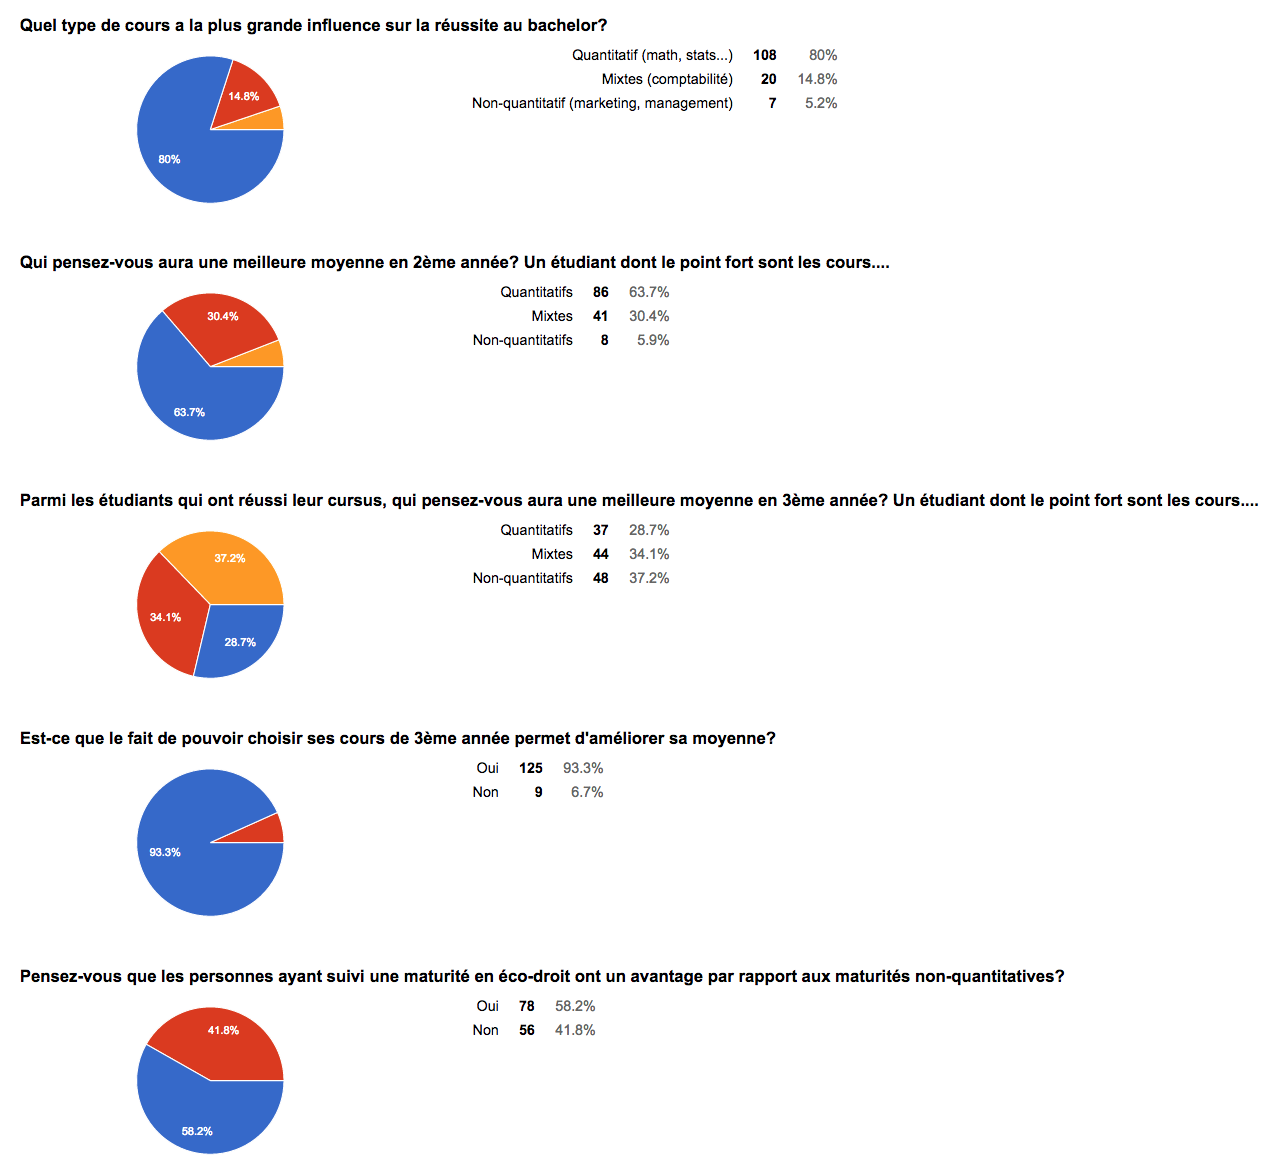
\includegraphics[width=0.9\paperwidth]{img/sondage1.png}}
\caption{Résultats de notre sondage}
\label{fig:sondage1}
\end{figure}

\vfill
\pagebreak

\begin{figure}[H]
\makebox[\textwidth][c]{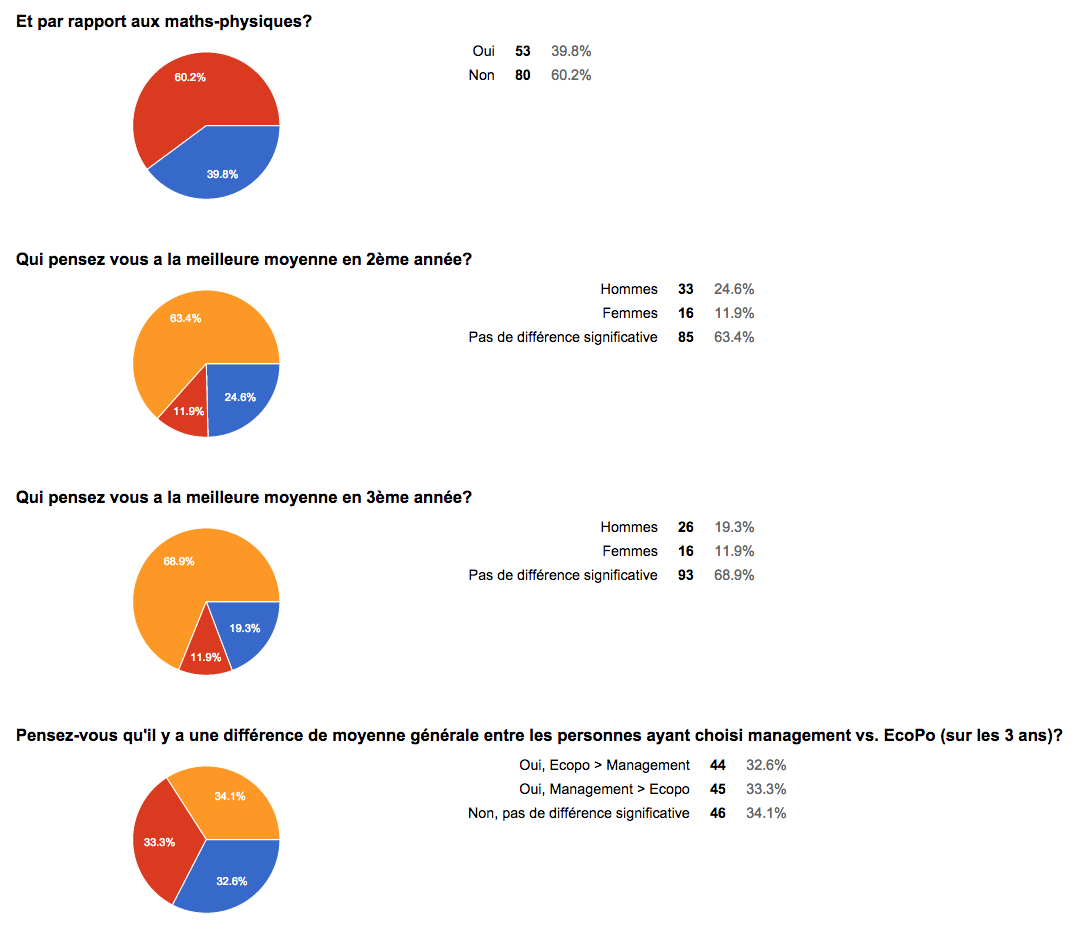
\includegraphics[width=0.9\paperwidth]{img/sondage2.png}}
\caption{Résultats de notre sondage (suite)}
\label{fig:sondage2}
\end{figure}

